\documentclass[10pt]{beamer}
\usetheme[
%%% options passed to the outer theme
%    hidetitle,           % hide the (short) title in the sidebar
%    hideauthor,          % hide the (short) author in the sidebar
%    hideinstitute,       % hide the (short) institute in the bottom of the sidebar
%    shownavsym,          % show the navigation symbols
%    width=2cm,           % width of the sidebar (default is 2 cm)
%    hideothersubsections,% hide all subsections but the subsections in the current section
%    hideallsubsections,  % hide all subsections
%    left                % right of left position of sidebar (default is right)
  ]{Aalborg}
  
% If you want to change the colors of the various elements in the theme, edit and uncomment the following lines
% Change the bar and sidebar colors:
%\setbeamercolor{Aalborg}{fg=red!20,bg=red}
%\setbeamercolor{sidebar}{bg=red!20}
% Change the color of the structural elements:
%\setbeamercolor{structure}{fg=red}
% Change the frame title text color:
%\setbeamercolor{frametitle}{fg=blue}
% Change the normal text color background:
%\setbeamercolor{normal text}{bg=gray!10}
% ... and you can of course change a lot more - see the beamer user manual.

\usepackage[utf8]{inputenc}
\usepackage[english]{babel}
\usepackage[T1]{fontenc}
% Or whatever. Note that the encoding and the font should match. If T1
% does not look nice, try deleting the line with the fontenc.
\usepackage{helvet}


% colored hyperlinks
\newcommand{\chref}[2]{%
  \href{#1}{{\usebeamercolor[bg]{Aalborg}#2}}%
}

\title[Semantic Web Mining]% optional, use only with long paper titles
{Semantic Web Mining}

\subtitle{Semantic Web Course}  % could also be a conference name

\date{\today}

\author[Ali Mohebbi, Mehdi Keshani] 
 % optional, use only with lots of authors
{
  Ali Mohebbi\\
  \href{mailto:a.mohebbi@ce.sharif.edu}{{\tt a.mohebbi@ce.sharif.edu}}\\
   Mehdi Keshani\\
  \href{mailto:keshani@ce.sharif.edu}{{\tt keshani@ce.sharif.edu}}
}

% - Give the names in the same order as they appear in the paper.
% - Use the \inst{?} command only if the authors have different
%   affiliation. See the beamer manual for an example

\institute[
%  {\includegraphics[scale=0.2]{aau_segl}}\\ %insert a company, department or university logo
  Dept.\ of Computer Engineering\\
  Sharif University\\
  Iran
] % optional - is placed in the bottom of the sidebar on every slide
{% is placed on the bottom of the title page
  Dept.\ of Computer Engineering\\
  Sharif University\\
  Iran
  
  %there must be an empty line above this line - otherwise some unwanted space is added between the university and the country (I do not know why;( )
}

% specify the logo in the top right/left of the slide
\pgfdeclareimage[height=1cm]{mainlogo}{AAUgraphics/aau_logo_new} % placed in the upper left/right corner
\logo{\pgfuseimage{mainlogo}}

% specify a logo on the titlepage (you can specify additional logos an include them in 
% institute command below
\pgfdeclareimage[height=1.5cm]{titlepagelogo}{AAUgraphics/aau_logo_new} % placed on the title page
%\pgfdeclareimage[height=1.5cm]{titlepagelogo2}{AAUgraphics/aau_logo_new} % placed on the title page
\titlegraphic{% is placed on the bottom of the title page
  \pgfuseimage{titlepagelogo}
%  \hspace{1cm}\pgfuseimage{titlepagelogo2}
}

\begin{document}
% the titlepage
{\aauwavesbg
\begin{frame}[plain,noframenumbering] % the plain option removes the sidebar and header from the title page
  \titlepage
\end{frame}}
%%%%%%%%%%%%%%%%

% TOC
\begin{frame}{Agenda}{}
\tableofcontents
\end{frame}
%%%%%%%%%%%%%%%%


\section{Data Mining}
\subsection{Classification}
\begin{frame}{Data Mining}{Classification}

\end{frame}
\subsection{Clustring}
\begin{frame}{Data Mining}{Clustering}

\end{frame}
\subsection{Association Rule Mining}
\begin{frame}{Data Mining}{Association Rule Mining}

\end{frame}
\section{Semantic Web Mining}
\subsection{Classification}
\begin{frame}{Semantic Web Mining}{Classification}

\end{frame}
\subsection{Clustring}
\begin{frame}{Semantic Web Mining}{Clustering}

\end{frame}
\subsection{Association Rule Mining}
\begin{frame}{Semantic Web Mining}{Association Rule Mining}
\end{frame}

\section{Association Rule Mining}
\subsection{Challenges}
\begin{frame}{Association Rule Mining}{Challenges}


\end{frame}
\subsection{Related Works}
\begin{frame}{Association Rule Mining}{Related Works}
\begin{itemize}
\item salam
\item hi
\end{itemize}

\begin{figure}[H]
	\centering
	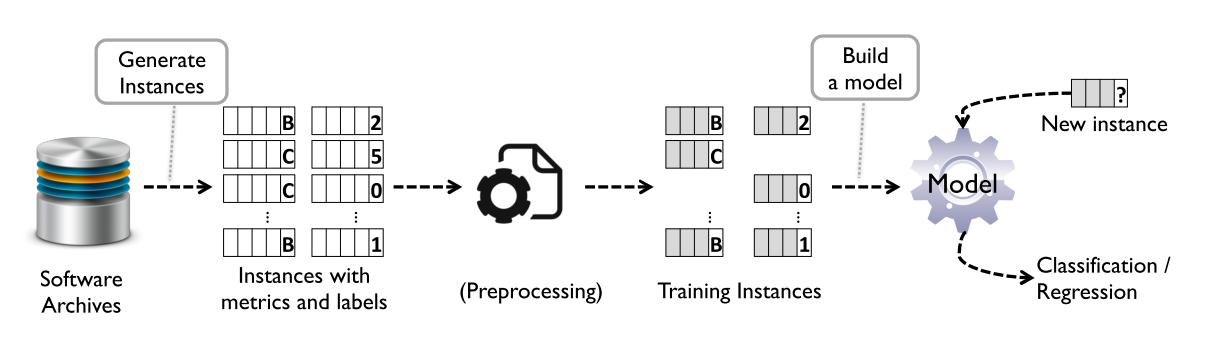
\includegraphics[width=1.0\textwidth]{images/prediction-process.PNG}
	\caption{process \cite{nam2014survey}}
	\label{fig:prediction-process}
\end{figure}

\end{frame}

\section{References}
 \begin{frame}[allowframebreaks] {References}
 \bibliographystyle{plain}
\bibliography{References}
\end{frame}
%%%%%%%%%%%%%%%%

{\aauwavesbg%
\begin{frame}[plain,noframenumbering]%
  \finalpage{Thank you.}
\end{frame}}
%%%%%%%%%%%%%%%%

\end{document}
